\documentclass[a4paper,12pt,twoside]{article}

\usepackage{../IyA.estilo.2015}
\usepackage{acronym}
\usepackage{caption}
\usepackage{enumerate}

%-------------------para incluir archivos graficos .gif------%
\epstopdfDeclareGraphicsRule{.gif}{png}{.png}{%
  convert gif:#1 png:\OutputFile
}
\AppendGraphicsExtensions{.gif}



%------------------Define box and box title style
\tikzstyle{mybox} = [draw=red, fill=yellow!20, very thick,
    rectangle, rounded corners, inner sep=10pt, inner ysep=20pt]
\tikzstyle{fancytitle} =[fill=blue!80, text=white]

\tikzstyle{grupos} = [draw=blue, fill=green!20, very thick,
    rectangle, rounded corners, inner sep=10pt, inner ysep=20pt]
\tikzstyle{fancytitle.grupos} =[fill=blue, text=white, ellipse]


\newcommand{\fullref}[1]{\ref{#1} de la p\'agina \pageref{#1}}

%-------------------------------------Encabezado
\fancyhead[RO,LE]{\small{{\bf \large Instrumentos y Avi\'onica} \\
\textcolor{blue}{\bf Directores de vuelo}\\
P\'agina \thepage \ de \pageref{LastPage}
                 }
                 }

\fancyhead[RE,LO]{
	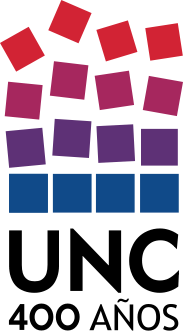
\includegraphics[height=1.5cm]{../imagenes/UNC-400-anios.png}
	
\includegraphics[height=1.2cm]{../imagenes/logo.jpg}
	
\includegraphics[height=1.2cm]{../imagenes/fcefyn.png}
	
\includegraphics[height=1.2cm]{../imagenes/dpto-aero-logo.jpg}
}

%----------------------------------Caratula
\title{Directores de vuelo}
\author{Ing. Jorge Garcia (jgarcia@efn.uncor.edu)}
\date{\today}

\begin{document}

\renewcommand{\tablename}{Tabla}

\newcommand{\ESPACIO}{\rule{0in}{3ex}}

\thispagestyle{fancy}
\maketitle

\thispagestyle{fancy}
\tableofcontents


\section{Finalidad y operaci\'on}
\label{sec:finalidad.y.operacion}


Estos sistemas tienen como finalidad dirijir al piloto para que este efect\'ue en forma correcta las maniobras de vuelo seg\'un el modo de operaci\'on elejido, adem\'as cumple las funciones b\'asicas de indicaci\'on de actitud y rumbo.

Existen diferentes tipos de directores de vuelo en cuanto a la forma de 
indicaci\'on y selecci\'on de modos pero cumplen la misma funci\'on.

\section{Componentes de cabina}
\label{sec:componentes.cabina}

\subsection{Indicador y Director de Actitud (ADI)}
\label{sec:adi}

Este instrumento posee una esfera indicadora de actitud y punteros de 
mando (lateral y vertical), que dan al piloto la informaci\'on requerida
para interceptor y mantener una determinada senda de vuelo que, junto
con sus dem\'as componentes, son:

\begin{enumerate}[(a)]
	\item \textbf{Esfera de actitud: }
        \item Avi\'on simb\'olico en miniatura
        \item Indice de actitud en alabeo
        \item Barras de mando
        \item Escala de senda de planeo
        \item Barras de mando
        \item Escala de senda de planeo
        \item Barra de radio altura
        \item Localizador expandido
        \item Inclin\'ometro
        \item Perilla de ajuste de actitud en cabeceo
        \item Pulsador de prueba de actitud
        \item Llave de erecci\'on r\'apida del gir\'oscopo vertical
          

\end{enumerate}


\subsection{Indicador de Situaci\'on Horizontal (HSI)}
\label{sec:indicador.situacion.horizontal}

Este instrumento provee adem\'as de la indicaci\'on de rumbo del avi\'on
una indicaci\'on pictogr\'afica que representa la posici\'on
del avi\'on respecto a un localizador VOR, y una indicaci\'on de la
posici\'on del avi\'on respecto a la senda de planeo.

La descripci\'on de cada uno de sus componentes:

\begin{enumerate}{\bf a)}
	\item {\bf S\'imbolo del avi\'on:} se encuentra fijo e indica la
		posici\'on de la aeronave respecto a un curso de radio
		y a un cuadrante m\'ovil indicador del rumbo. Esta fijado
		al vidrio del instrumento.
        \item {\bf Cuadrante rotante de rumbo:}
        \item {\bf \'Indice principal de rumbo:}
        \item {\bf Marcas de azimut:}
        \item {\bf \'Indice y perilla de rumbo selectado:}
        \item {\bf Puntero y perilla de curso:}
        \item {\bf Barra de desviaci\'on de curso:}
        \item {\bf Puntos de desviaci\'on de curso:}
        \item {\bf Indicador de ``\emph{hacia-de}'' }
        \item {\bf Disco m\'ovil de curso:}
        \item {\bf \'Indice y puntos de desviaci\'on de senda de planeo:}
        \item {\bf Anunciador de sincronismo:}
        \item {\bf Llave de ``\emph{Esclavo-Libre}'':}
        \item {\bf Llave de incremento (INC) - decrecimiento (DEC):}

\end{enumerate}

\subsection{Control - Computador}
\label{sec:control.computador}

Este elemento combina los datos de rumbo, actitud, altitud y receptor de 
navegaci\'on en se\~nales computadas que comandar\'an las barras
directoras del ADI.
Contiene en su frente los botones por medio de los cuales se
seleccionan el o los modos de operaci\'on deseados.

Los modos que se encuentran en operaci\'on son enunciados al iluminarse
el bot\'on correspondiente.


FIGURA TECLADO

\section{Modos de operaci\'on}
\label{sec:modos.operacion}

Este sistema utiliza los datos de VOR-Localizadores y de Senda de Planeo,
proporcionados por los receptores de navegaci\'on corrientes.
Utiliza tambi\'en datos de altitud de un sensor de altura barom\'etrico
propio (adem\'as del de sistema de radio-alt\'imetro), datos de rumbo
desde un gir\'oscopo direccional y de actitud desde un gir\'oscopo
vertical, elementos estos que pertenecen al mismo sistema.

Todas estas informaciones son computadas siendo finalmente enviado su
resultado a comandar las barras directoras del sistema para guiar al
piloto en las maniobras que debe efectuar, para mantener o tomar la
senda de vuelo selectada, tanto para la navegaci\'on como para la
aproximaci\'on de aterrizaje.

Los modos de operaci\'on que puede selectar el piloto son los siguientes:

%\begin{multicols}
  \begin{tabular}{lm{3mm}l}
    	SBY &  & Preparado \\
	GO AROUND &  & Escape \\
	ALT &  & Mantenimiento de altura    \\
	PAT &  & Ajuste de actitud en cabeceo \\
	HDB &  & Rumbo selectado \\
	V/L &  & VOR - Localizador \\
        GS ARM & & Armado Pendiente de Planeo \\
	GS & & Pendiente de Planeo \\
	GS EXT & &  \\
	REV & & Curso opuesto \\
  \end{tabular}
%\end{multicols}

\subsubsection{Modo Preparado (SBY)}
\label{sec:modo.sby}

\subsubsection{Modo Ajuste Actitud de Cabeceo (Pitch Attitude Trim, PAT)}
\label{sec:modo.ajuste.pitch}

\subsubsection{Modo Rumbo Selectado (Heading HDG)}
\label{sec:hdg}

\subsubsection{Modo mantenimiento de altura (ALT)}
\label{sec:alt}

\subsubsection{Modo Escape (GO AROUND)}
\label{sec:go.araund}

\subsubsection{Modo VOR - Localizador (	V/L )} \\
\label{sec:VL}

\subsubsection{Armado Pendiente de Planeo}
\label{sec:GS.arm}

\subsubsection{Pendiente de Planeo}
\label{sec:gs}

\subsubsection{Modo anunciador ampliaci\'on de indicaci\'on en pendiente de planeo (GS EXT)}
\label{sec:gs.ext}

\subsubsection{Modo Curso Opuesto (REV)}
\label{sec:rev}


\section{Incorporaci\'on del sistema de radioalt\'imetro}
\label{sec:incorporacion.sistema.radio.altimetro}

El radioalt\'imetro provee una indicaci\'on de altura absoluta en un indicador,
pero adem\'as se interconecta con el director de vuelo a los fines
de manejar la barra de radioaltura en el ADI.

Cuando el sistema de radioalt\'imetro funciona, la barra de radioaltura aparece a la vista
en la parte inferior del instrumento a los 61 (sesenta y un) metros y, a medida que
el avi\'on se acerca a tierra, esta barra sube simulando el acercamiento de la aeronave
a tierra mediante el acercamiento relativo del avi\'on miniatura del ADI
a la barra en miniatura que simula el terreno.

Al tocar tierra la aeronave, la barra de altura del instrumento toca la parte
inferior del avi\'on simb\'olico del ADI.

El sistema de radioaltimetro est\'a compuesto por dos (2) antenas, una transmisora
y otra receptora, un transceptor y un indicador.
Su principio de funcionamiento se basa en la emisi\'on de ondas de UHF, moduladas
en frecuencia, por la antena transmisora, las cuales son reflejadas por la superficie
terrestre y receptadas por la segunda antena. La diferencia de frecuencia entre
las ondas emitidas y las reflejadas es representativa de la altura a la cual se
encuentra la aeronave del suelo, y es indicada en el instrumento.

En otros sistemas se utiliza la modulaci\'on de pulsos.



\end{document}
